\chapter{Notes on Camera Calibration and Transformations}
\label{computervision}


\section{Simplified Perspective Transform}
To extract spatial information from camera images, we need to derive equations to compute an object's coordinates in the world frame $(x,y,z)_w$ 
based on row and column pixel coordinates in the image $(r,c)_c$.  Instead of giving you these equations, this section will walk through how the transform works to allow you to derive them yourself.

\begin{figure}[ht]
	\centering
		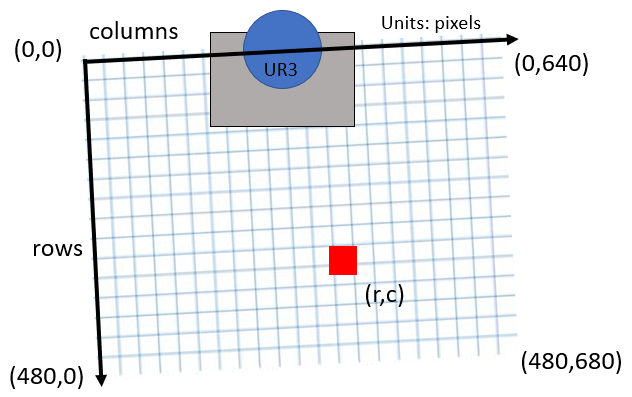
\includegraphics[height=6cm]{image/appendixC_camera_1.png}
	\caption{\figlbl{cam_1} The view from the camera.}
\end{figure}

The image starts as seen in \figref{cam_1}.  We can see that all data is in pixels, so the location of the object would be described by the rows and columns of the pixel at the centroid of the red block.  We can further see that the image is not square to the table, but instead slightly rotated.  We will ignore that for the time being.

\begin{figure}[ht]
	\centering
		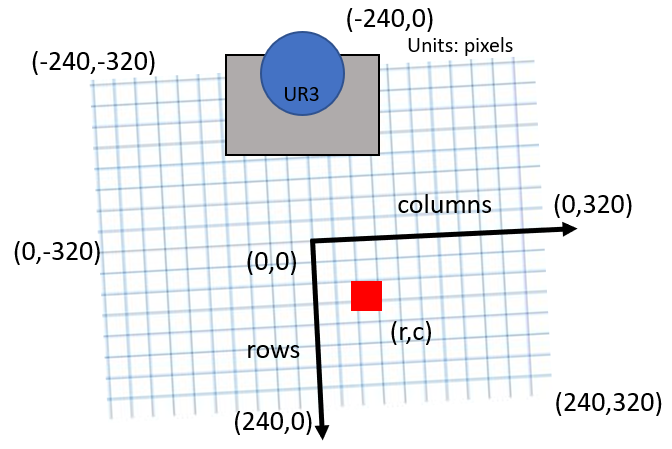
\includegraphics[height=6cm]{image/appendixC_camera_2.png}
	\caption{\figlbl{cam_2}  The view from the camera with the origin shifted to the principal point.}
\end{figure}
The first step is to translate the frame from the top left corner, to the center of the image also known as the principal point as seen in \figref{cam_2}.  As seen in Table \ref{tab:DOV}, the location of the principal point is in our original frame are called $\left(O_{r},O_{c}\right)$.  Based on this image, what are $O_{r}$ and $O_{c}$

\begin{eqnarray*}
	O_{r} & = & \\
	O_{c} & = &
\end{eqnarray*}
Side note: It is possible to develop the camera transformation without this translations, but shifting to the principle point is the standard method.  It is recommended that you consult a more exhaustive text on computer vision to better understand why.

The next step is to move from pixel measurements to something we can measure in the real world such as meters.  To do this, we need a relationship between pixel distance and physical distance on the table top. This value depends both on the physical properties of the camera and the distance between the camera and table top.  The physical properties of the camera are encapsulated by focal length ($f_{x}$ and $f_{y}$ as seen in Table \ref{tab:DOV}).  Because we do not know the focal length of the camera, we instead create a simple value $\beta$ which encapsulates both pieces of information:
\[
\beta=\frac{f_x}{z_c}=\frac{f_y}{z_c}. 
\]
This is a simplification of this relationship.  It assumes that pixels are square and that the lens does not distort the image at all.  Because of this, you might find it is less accurate at the edges of the image, but it should work fine for our purposes.  The units of $\beta$ are pixels per meter.

We now have enough information to complete our first equation.  This equation gives us the location of the block in meters, but with respect to the camera frame and not the world frame.  These equations are often called the \textbf{intrinsic} equations because they rely on the intrinsic properties of the camera such as $O_{r}$, $O_{c}$, $f_{x}$ and $f_{y}$ (i.e. properties that don't change).  These equations are essentially a transition from the camera sensor to the tabletop as seen in \figref{cam_3}.  Please complete the intrinsic equations using only $\beta$, $O_{r}$, and $O_{c}$
\begin{eqnarray*}
	x_c(r) & = & \\
	y_c(c) & = &
\end{eqnarray*}

\begin{figure}[ht]
	\centering
		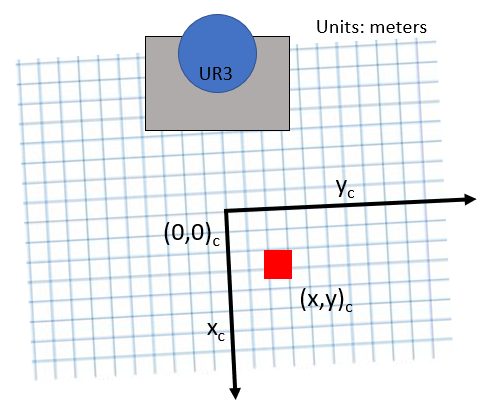
\includegraphics[height=6cm]{image/appendixC_camera_3.png}
	\caption{\figlbl{cam_3} The camera frame projected onto the table top.  This is the output of the intrinsic equations.}
\end{figure}


Now that we have the intrinsic equations and have transitioned to the table top, we can try to align this table top camera frame with the world frame at the corner of the aluminum plate.  We start this by shifting the frame from its current position which sits where the principal point lines up on the table top as shown in \figref{cam_4}.  As seen in Table \ref{tab:DOV}, the relationship between these two frames is $O_{cw}$ which is the origin of the world frame in terms of the camera frame.  The key values here are $T_{x}$ and $T_{y}$ as $T_{z}=0$.



\begin{figure}[ht]
	\centering
		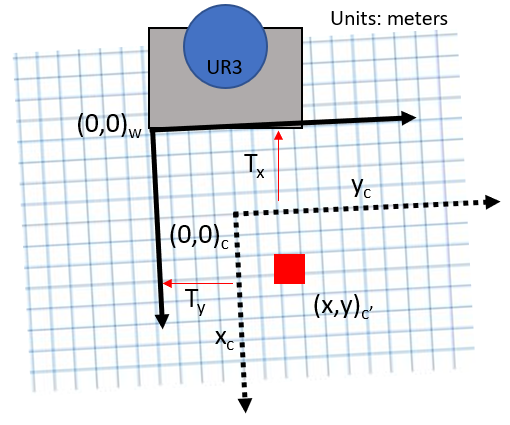
\includegraphics[height=6cm]{image/appendixC_camera_4.png}
	\caption{\figlbl{cam_4} The table top camera frame must be translated to align with the world frame.}
\end{figure}

Now that we have aligned the origins, it is time to straighten up the frame as shown in \figref{cam_5}.  We do this naturally by a rotation about the z-axis by the angle $\theta$.  We can see in Table \ref{tab:DOV} that $\theta$ is defined for $R_{cw}$.


\begin{figure}[ht]
	\centering
		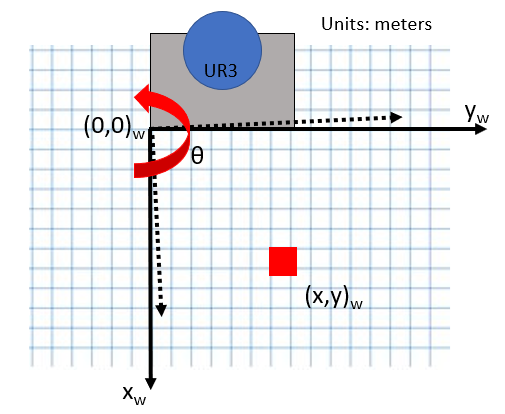
\includegraphics[height=6cm]{image/appendixC_camera_5.png}
	\caption{\figlbl{cam_5} The table top camera frame must be rotated to align with the world frame.}
\end{figure}


Now that we have translated and rotated our frame to align with the world frame, we can write the \textbf{extrinsic} equations.  These are known as extrinsic equations because they are based on values outside of the camera and change depending on placement and orientation.  Let's write the extrinsic equations:

\[
\left[\begin{array}{c}
x_w \\ y_w
\end{array}\right] = 
\]



Pay special attention to the signs of $T_{x}$ and $T_{y}$! 

We now have both the intrinsic and extrinsic equations and we can put them both together:

\begin{eqnarray*}
	x_w(r,c) & = & \\
	y_w(r,c) & = &
\end{eqnarray*}

These are the equations that you will use in your code to perform the camera transformation.  What about $z_w$?  Well, since we are working on the flat table top, $z_w$ is just the height of any object we wish to pick up.  A value for $z_w$ is provide in the code.

\begin{table}
	\centering
	\begin{tabular}{cl}
			Name & Description \\
		  \hline
			$(r,c)$     & (row,column) coordinates of image pixel \\
			$f_x,f_y$ & ratio of focal length to physical width and length of a pixel \\
			$(O_r,O_c)$ & (row,column) coordinates of {\it principal point} of image\\
            & (principal point of our image is center pixel) \\
			$(x_c,y_c)$ & (meters) coordinates of point in camera frame \\
% 			$p^c$	    & = $[x^c y^c z^c]^T$coordinates of point in camera frame \\
% 			$p^w$	    & = $[x^w y^w z^w]^T$coordinates of point in world frame \\
			$O_{cw}$		& = $[T_x T_y T_z]^T$ origin of world frame expressed in camera frame \\
			$R_{cw}$     & rotation expressing world frame w.r.t. camera frame. \\
		  \hline
	\end{tabular}
	\caption{Definitions of variables necessary for camera calibration.}
	\label{tab:DOV}
\end{table}


\section{Camera Calibration}
After formulating the camera transformation it is natural to ask how the key values such as $\beta$, $\theta$, $T_{x}$ and $T_{y}$ are found.  This is through the process of camera calibration.  Due to simulation limitations, this has already been done for this lab.  This section will give a brief introduction to how this process works.
\begin{itemize}
    \item $\beta$ - This value is found using a calibration stick.  The stick has two target set 10cm apart (center to center).  When the centroids of these targets are found, their distance in pixels can be determined.  It is then just a matter of relating the pixels to the fixed 10cm distance.
    \item $\theta$ - The same calibration stick is used again.  It is placed on the table top such that it carefully aligns with the y-axis of the world frame.  When the centroids of the targets are found, a right triangle can be formed with the two points and the angle formed will be $\theta$.
    \item $T_{x}$ and $T_{y}$ - This time a single target is placed on the table top with a known position in the world frame.  With this known positions, the location of the centroid (r,c) and $\beta$ and $\theta$, the only unknown in the camera transformation equations are $T_{x}$ and $T_{y}$, which can easily be solved for.
\end{itemize}






